\subsection{User-manual documentation on k-degeneracy}
This section describes the idea of k-core and the implementation of analyzing the degeneracy of of a graph using SQL.\par

First, we look at the definition of coreness: (definitions come from project writeup) A node in an undirected graph has coreness k, if it has k or more neighbors that have coreness k or higher, and k is the maximum such integer for node n. After we know the coreness of each node in the graph, we can get the degeneracy of a graph. The formal definition is: Degeneracy D of a graph is the highest coreness among the nodes of thegraph.\par

Now we have seen the definition of degeneracy, so the general idea of finding the coreness of each node is described below: iterate from k = 1, and we want to find nodes whose coreness = k; for each k, find those nodes who has neighbors less than or equal to k, so those numbers are of coreness k; delete those nodes from the graph; repeat until we can not find any of the node who has neighbors $\le$ k, all the nodes left must have coreness greater than k, so we increase k by 1; terminate when there is no node in the graph.\par

Part of the SQL code are provided below:\par
\begin{lstlisting}
-- 1. start from k = 1, loop when we can still find nodes with neighbors <= k
--     create a temp table to store all nodes that we find with neighbors <= k
INSERT INTO TMP_TABLE
SELECT src_id, COUNT(*) AS neighbor FROM GM_TABLE
GROUP BY src_id HAVING count(*) <= k;
                 
-- 2. check if there is no nodes satisfying the conditions, increase k by 1 and continue from the start of the loop
SELECT COUNT(*) FROM TMP_TABLE;
-- if count is 0, k += 1 and continue

-- 3. save those nodes to a permanent table with their coreness
INSERT INTO GM_KCORE
SELECT src_id, k AS coreness FROM TMP_TABLE;

-- 4. delete those nodes from the original table
DELETE FROM GM_TABLE
WHERE src_id IN (SELECT src_id FROM TMP_TABLE);
DELETE FROM GM_TABLE
WHERE dst_id IN (SELECT src_id FROM TMP_TABLE);
	
-- 5. terminate if there is no node in the original table
SELECT COUNT(*) FROM GM_TABLE;
-- if count is 0, break the loop
		
-- 6. calculate the degeneracy of the graph, which is the largest coreness among all nodes
SELECT MAX(coreness) FROM GM_KCORE;
\end{lstlisting}

\subsection{Dataset}

Our datasets are adopted from SNAP (Stanford Large Network Dataset Collection) \\
\url{http://snap.stanford.edu/data/index.html}.

\begin{table}[H]
	\begin{tabular}{| l | l | l | l | p{8cm} |}
	  \hline			
	  dataset & Type & Nodes & Edges & Description \\ \hline

	  Facebook & Undirected & 4,039 & 88,234 & \textbf{Social network} Social circles from Facebook (anonymized) \\ \hline

	  soc-Slashdot0811 & Directed & 77,360 & 905,468 & \textbf{Social network} Slashdot social network from November 2008 \\ \hline

	  soc-Slashdot0922 & Directed & 82,168 & 948,464 & \textbf{Social network} Slashdot social network from February 2009 \\ \hline

	  soc-Epinions1 & Directed & 75,879	& 508,837 & \textbf{Social network} Who-trusts-whom network of Epinions.com \\ \hline

	  wiki-Vote	& Directed & 7,115 & 103,689 & \textbf{Wikipedia social network} Wikipedia who-votes-on-whom network \\ \hline

	  email-Enron & Undirected & 36,692 & 183,831 & \textbf{Communication network} Email communication network from Enron \\ \hline
	  
	  ca-HepTh & Undirected & 9,877	& 25,998 & \textbf{Collaboration network} of Arxiv High Energy Physics Theory \\ \hline

	  ca-GrQc & Undirected & 5,242 & 14,496 & \textbf{Collaboration network} of Arxiv General Relativity \\ \hline

	  ca-AstroPh & Undirected & 18,772 & 198,110 & \textbf{Collaboration network} of Arxiv Astro Physics \\ \hline

	  p2p-Gnutella24 & Directed & 26,518 & 65,369 & \textbf{P2P Network} Gnutella peer to peer network from August 24 2002 \\ \hline

	  p2p-Gnutella25 & Directed & 22,687 & 54,705 & \textbf{P2P Network} Gnutella peer to peer network from August 25 2002 \\ \hline

	  oregon1-010331 & Undirected & 10,670 & 22,002 & \textbf{Autonomous system} peering information inferred from Oregon route-views from March 31 \\ \hline

	  oregon1-010519 & Undirected & 11,051 & 22,724 & \textbf{Autonomous system} peering information inferred from Oregon route-views from May 19 \\ \hline

	  cit-HepPh & Directed & 34,546 & 421,578 & \textbf{Citation network} Arxiv High Energy Physics paper citation network \\ \hline

	  cit-HepTh & Directed & 27,770 & 352,807 & \textbf{Citation network} Arxiv High Energy Physics paper citation network \\
	  
	  \hline  
	\end{tabular}
\end{table}

\subsection{Results}

All the graphs shown below are in log-log scale.

\subsubsection{Degree Distribution}

Scatter plot \quad x-axis: degree \quad y-axis: count

\begin{figure}[H]
\minipage{0.33\textwidth}
  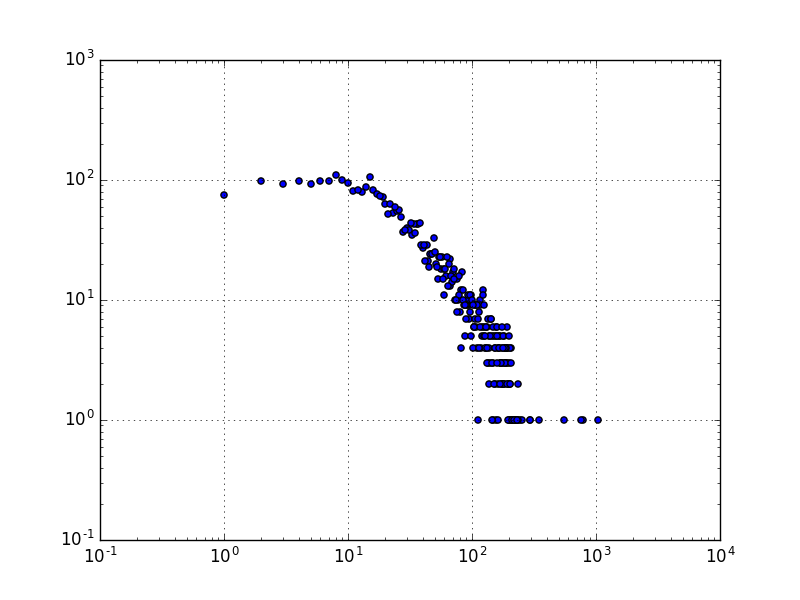
\includegraphics[width=\linewidth]{img/facebook/degree_dist.png}
  \caption*{Facebook}
\endminipage\hfill
\minipage{0.33\textwidth}
  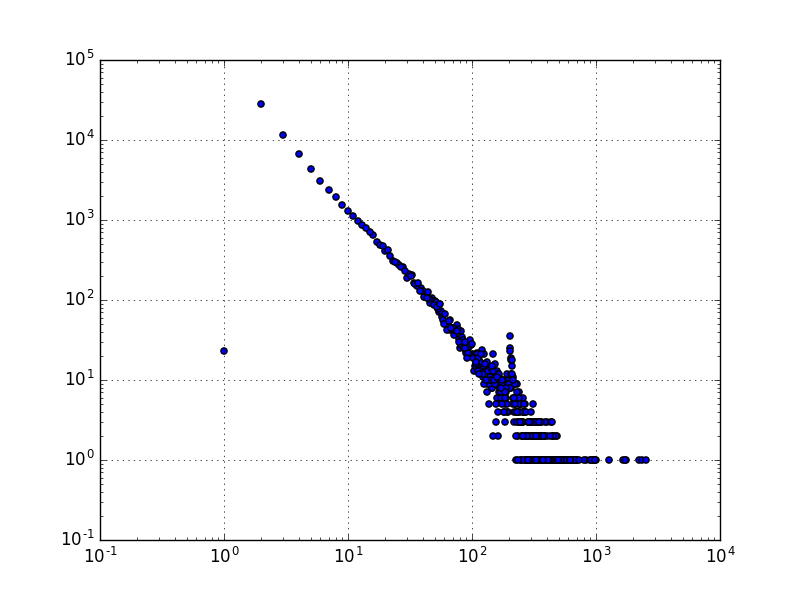
\includegraphics[width=\linewidth]{img/slashDot/degree_dist.png}
  \caption*{soc-Slashdot0811}
\endminipage\hfill
\minipage{0.33\textwidth}
  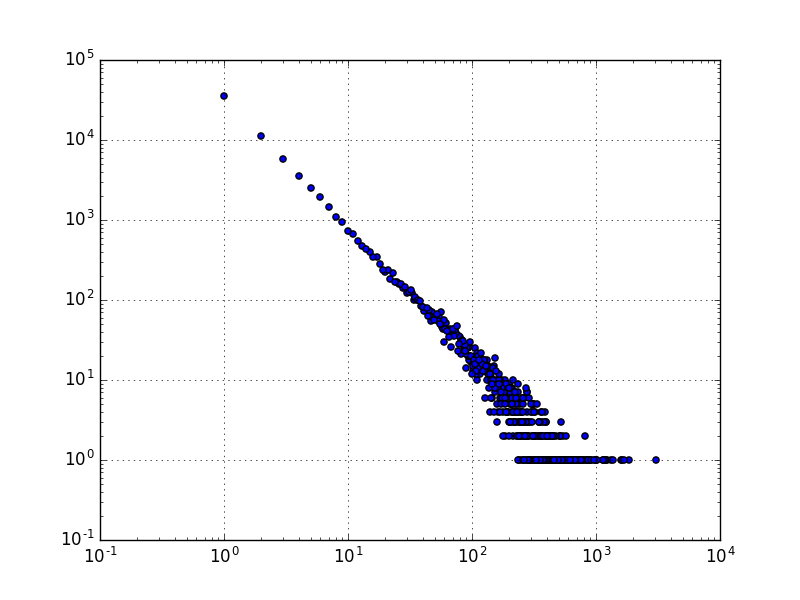
\includegraphics[width=\linewidth]{img/soc-E/degree_dist.png}
  \caption*{soc-Epinions1}
\endminipage
\end{figure}

\begin{figure}[H]
\minipage{0.33\textwidth}
  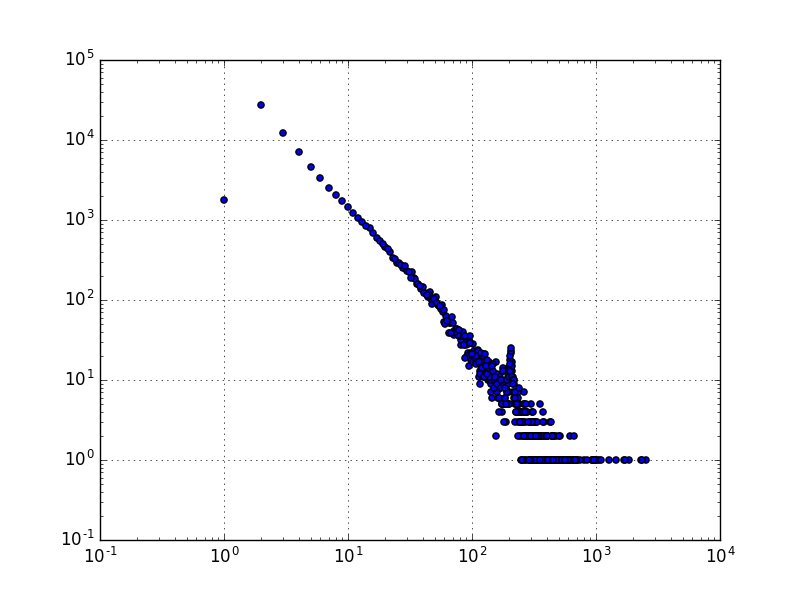
\includegraphics[width=\linewidth]{img/slashDot09/degree_dist.png}
  \caption*{soc-Slashdot0922}
\endminipage\hfill
\minipage{0.33\textwidth}
  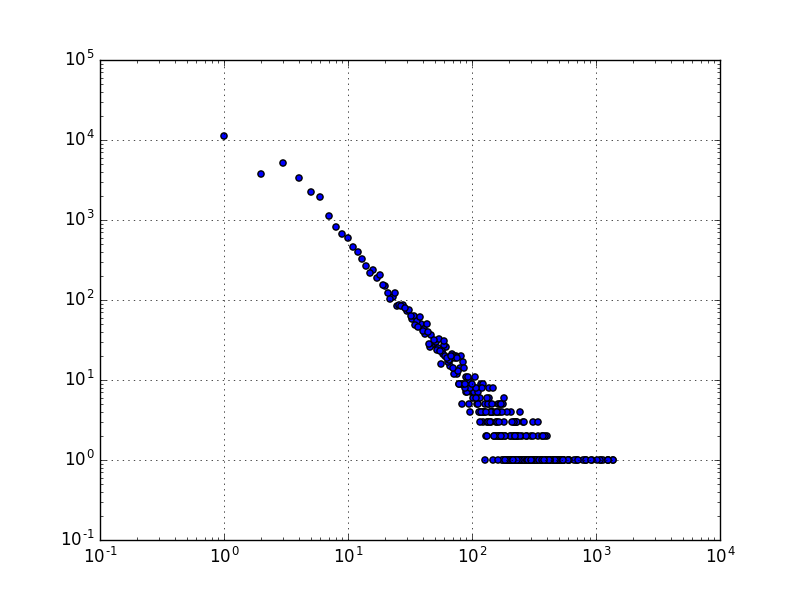
\includegraphics[width=\linewidth]{img/email/degree_dist.png}
  \caption*{email-Enron}
\endminipage\hfill
\minipage{0.33\textwidth}
  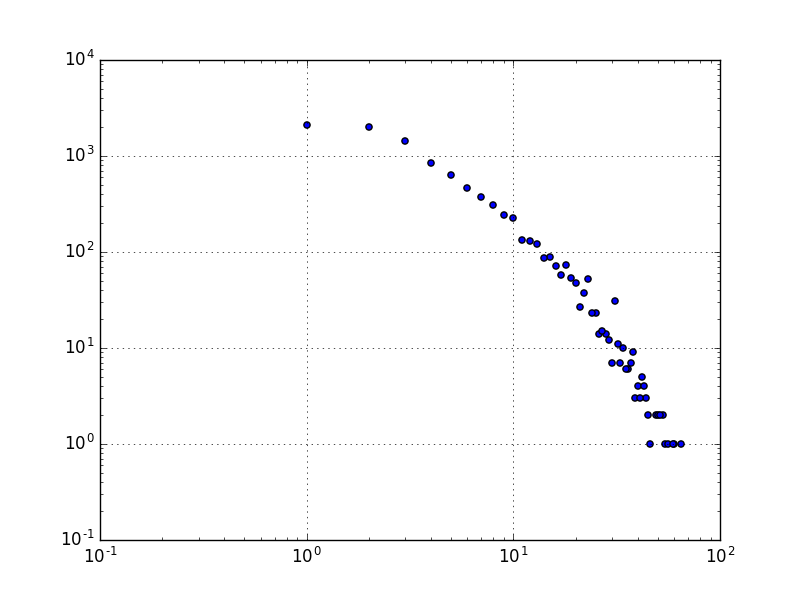
\includegraphics[width=\linewidth]{img/ca-HepTh/degree_dist.png}
  \caption*{ca-HepTh}
\endminipage
\end{figure}

\begin{figure}[H]
\minipage{0.33\textwidth}
  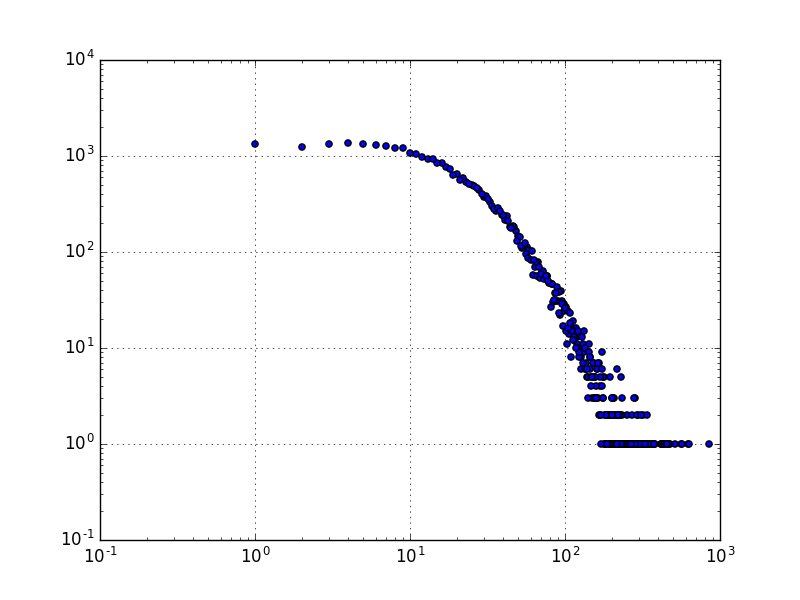
\includegraphics[width=\linewidth]{img/cit-HepPh/degree_dist.png}
  \caption*{cit-HepPh}
\endminipage\hfill
\minipage{0.33\textwidth}
  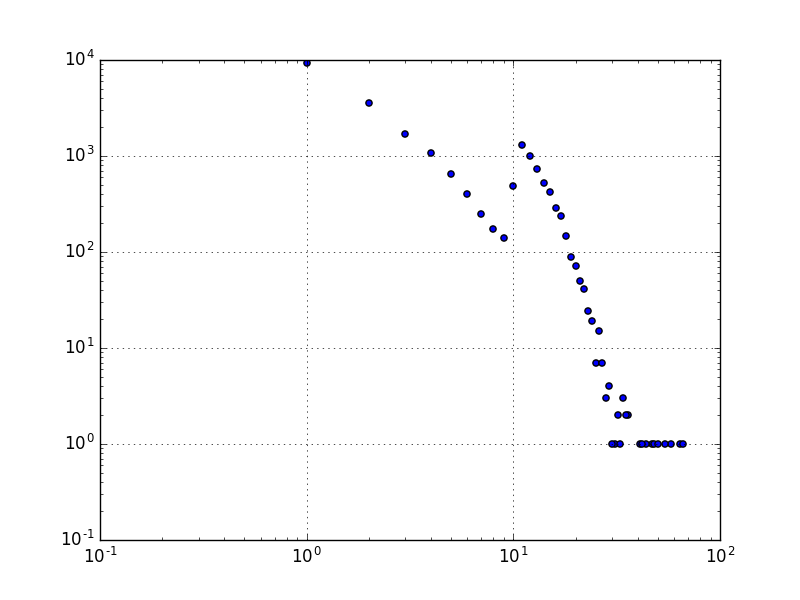
\includegraphics[width=\linewidth]{img/p2p-Gnutella25/degree_dist.png}
  \caption*{p2p-Gnutella25}
\endminipage\hfill
\minipage{0.33\textwidth}
  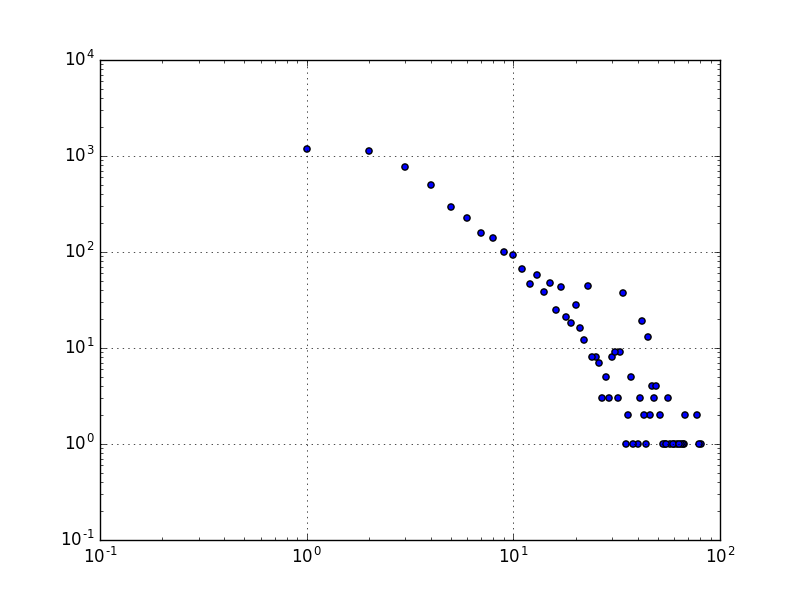
\includegraphics[width=\linewidth]{img/ca-GrQc/degree_dist.png}
  \caption*{ca-GrQc}
\endminipage
\end{figure}

\begin{figure}[H]
\minipage{0.33\textwidth}
  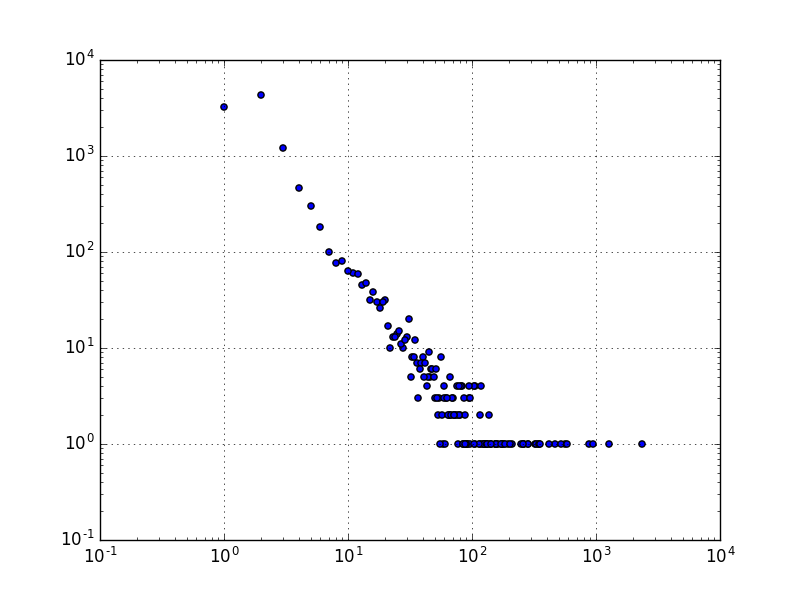
\includegraphics[width=\linewidth]{img/oregon-010331/degree_dist.png}
  \caption*{Oregon1-010331}
\endminipage\hfill
\minipage{0.33\textwidth}
  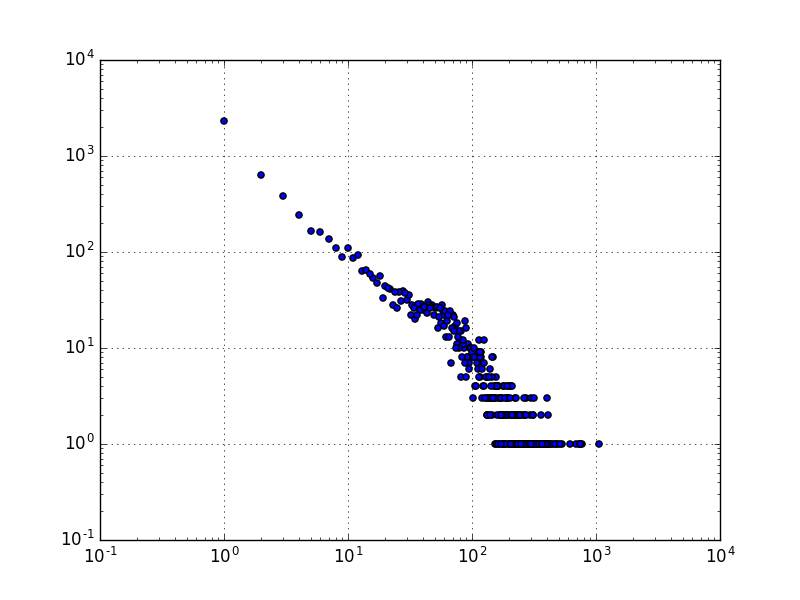
\includegraphics[width=\linewidth]{img/wiki-Vote/degree_dist.png}
  \caption*{wiki-Vote}
\endminipage\hfill
\minipage{0.33\textwidth}
  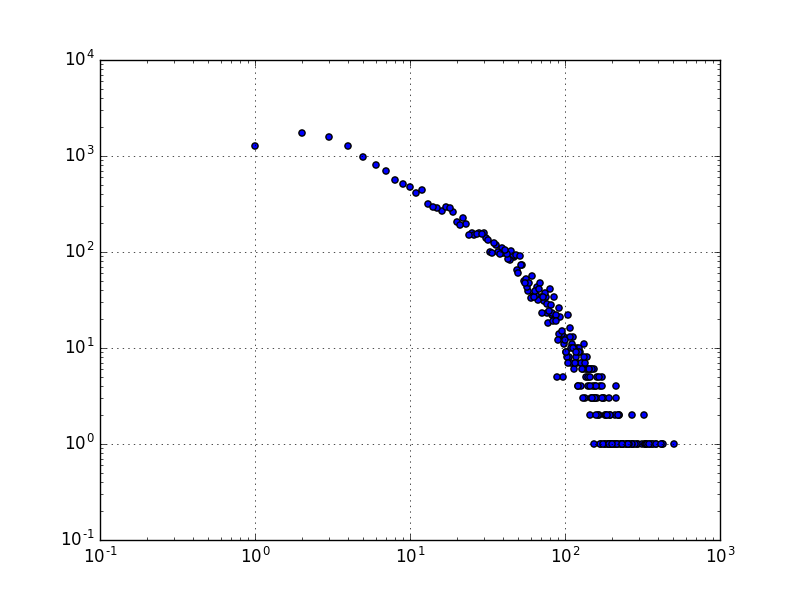
\includegraphics[width=\linewidth]{img/ca-Astro/degree_dist.png}
  \caption*{ca-Astro}
\endminipage
\end{figure}

\begin{figure}[H]
\minipage{0.33\textwidth}
  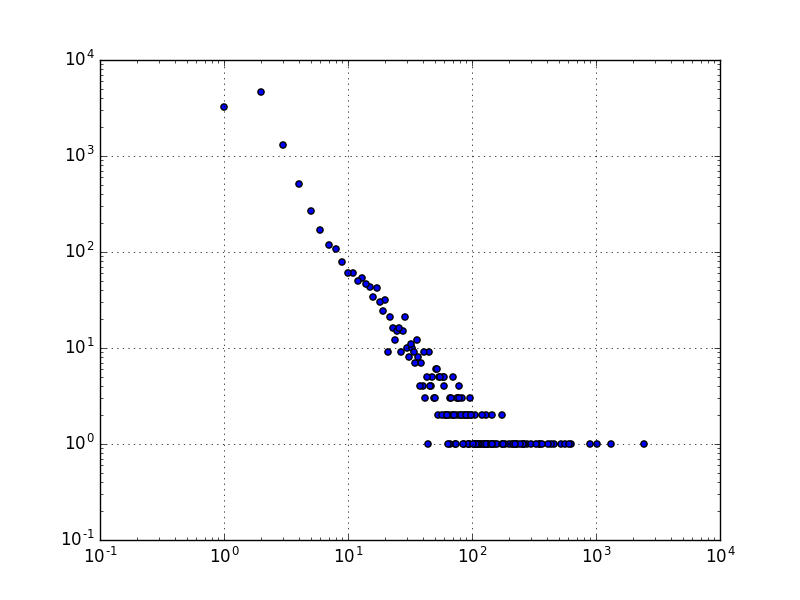
\includegraphics[width=\linewidth]{img/oregon-010519/degree_dist.png}
  \caption*{Oregon1-010519}
\endminipage\hfill
\minipage{0.33\textwidth}
  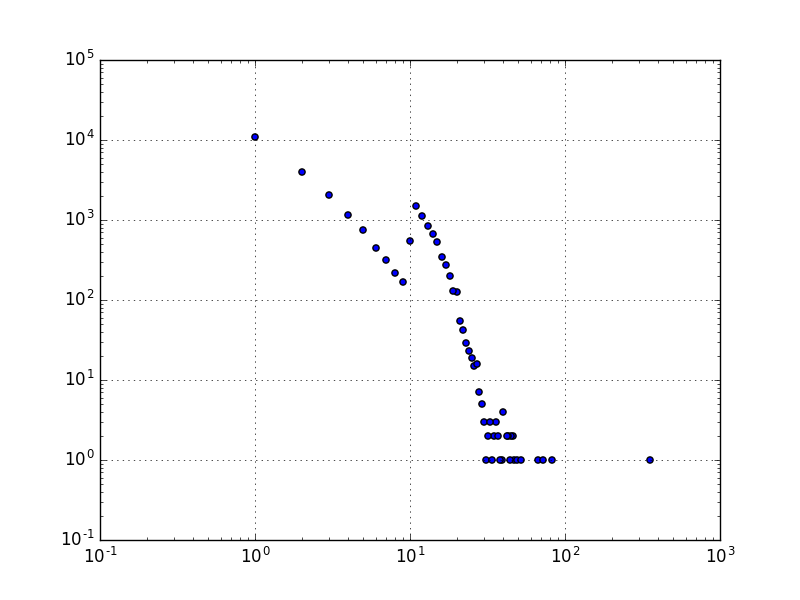
\includegraphics[width=\linewidth]{img/p2p-Gnutella24/degree_dist.png}
  \caption*{p2p-Gnutella24}
\endminipage\hfill
\minipage{0.33\textwidth}
  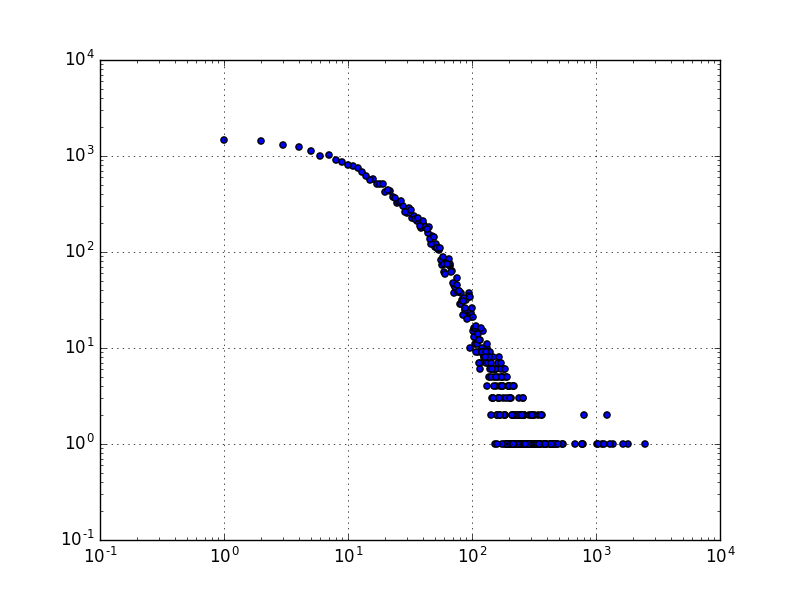
\includegraphics[width=\linewidth]{img/cit-HepTh/degree_dist.png}
  \caption*{cit-HepTh}
\endminipage
\end{figure}

Observations
\begin{itemize}
\item Most datasets exhibit a strong power law relation between degree and count. A large fraction of nodes (users) have very low degrees or very few connections. 
\item \textbf{P2P networks} (p2p-Gnutella24, pep-Gnutella25) exhibits a spike around degree = 10, implying that people tend to connect with 10 peers.
\item Some networks such as Facebook and \textbf{citation networks} do not follow a power law in degree range [1 - 10]. They look more like log-logistic. Taking Facebook for example, there are a lot of people with 1-10 friends, but the number of people with 1 friend and 10 friend does not differ much. Speaking in a formal way, nodes with a degree between 1 - 10 have similar counts.
\item We can also spot some outliers with only one connection in \{soc-Slashdot0811, soc-Slashdot0922\}, which probably means newly registered accounts in Slashdot Zoo, but they are less likely to get only one friend compared to the normal trend of other networks. Another outlier can be observed in dataset \{p2p-Gnutella 24\} where one node has a much higher degree = 200, probably because it functions as the central server in p2p network.
\end{itemize}

\subsubsection{Pagerank Distribution}

CCDF\quad x-axis: pagerank score \quad y-axis: count($\geq$ score)

\begin{figure}[H]
\minipage{0.33\textwidth}
  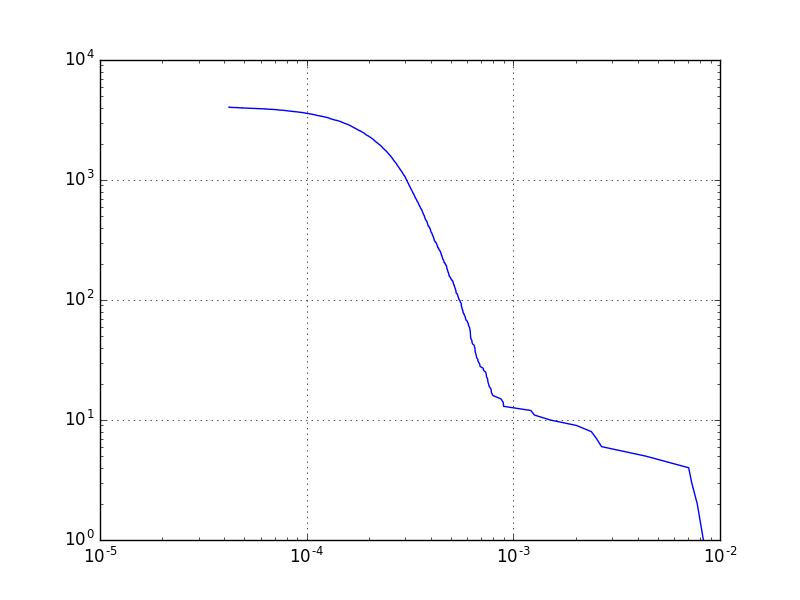
\includegraphics[width=\linewidth]{img/facebook/pagerank_ccdf.png}
  \caption*{Facebook}
\endminipage\hfill
\minipage{0.33\textwidth}
  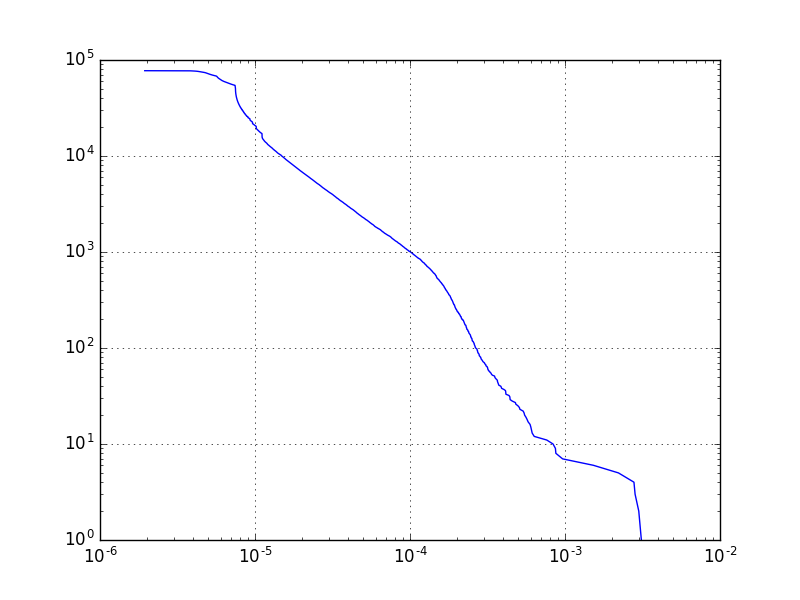
\includegraphics[width=\linewidth]{img/slashDot/pagerank_ccdf.png}
  \caption*{soc-Slashdot0811}
\endminipage\hfill
\minipage{0.33\textwidth}
  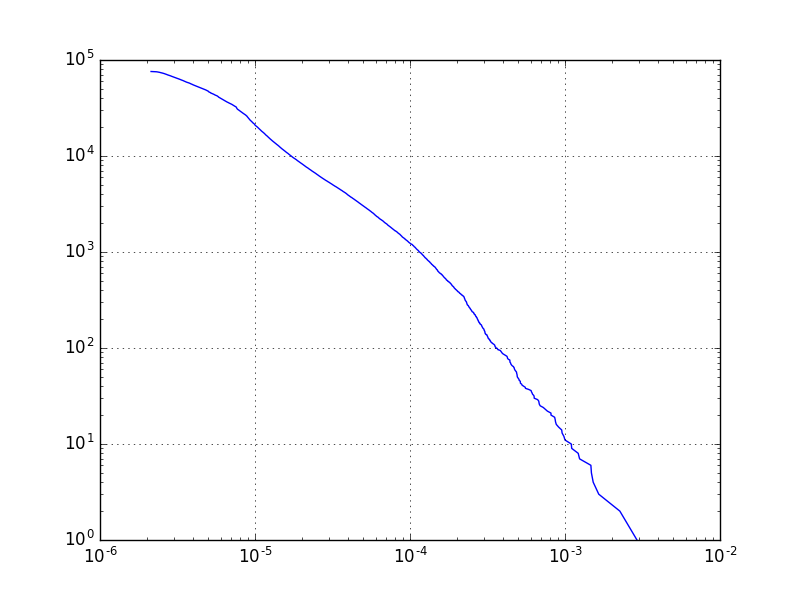
\includegraphics[width=\linewidth]{img/soc-E/pagerank_ccdf.png}
  \caption*{soc-Epinions1}
\endminipage
\end{figure}
\begin{figure}[H]
\minipage{0.33\textwidth}
  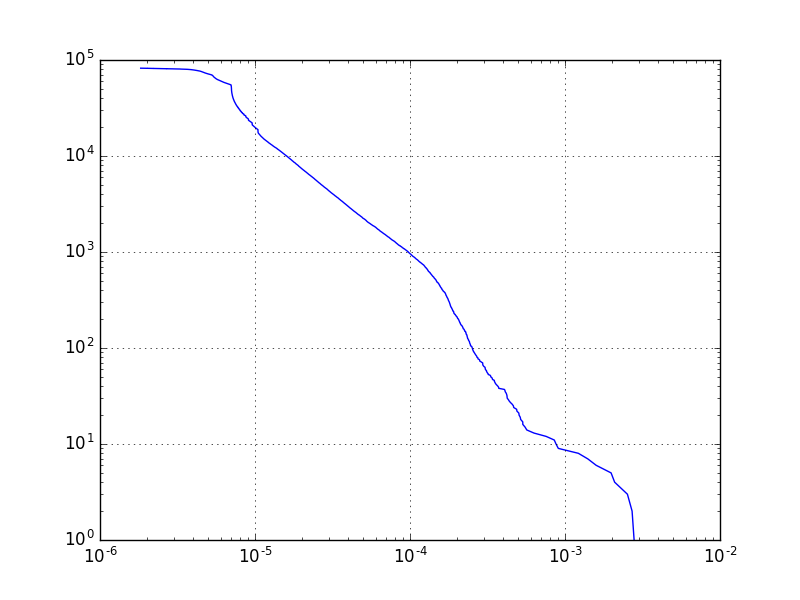
\includegraphics[width=\linewidth]{img/slashDot09/pagerank_ccdf.png}
  \caption*{soc-Slashdot0922}
\endminipage\hfill
\minipage{0.33\textwidth}
  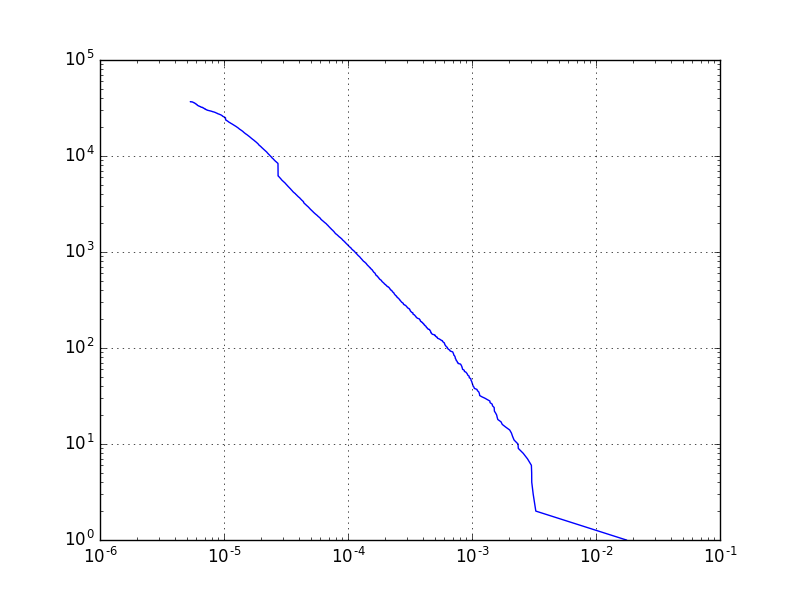
\includegraphics[width=\linewidth]{img/email/pagerank_ccdf.png}
  \caption*{email-Enron}
\endminipage\hfill
\minipage{0.33\textwidth}
  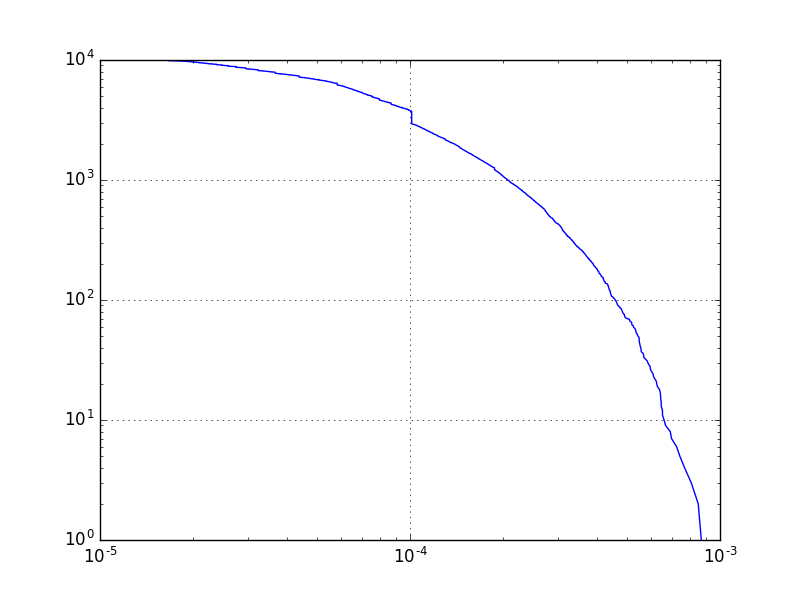
\includegraphics[width=\linewidth]{img/ca-HepTh/pagerank_ccdf.png}
  \caption*{ca-HepTh}
\endminipage
\end{figure}
\begin{figure}[H]
\minipage{0.33\textwidth}
  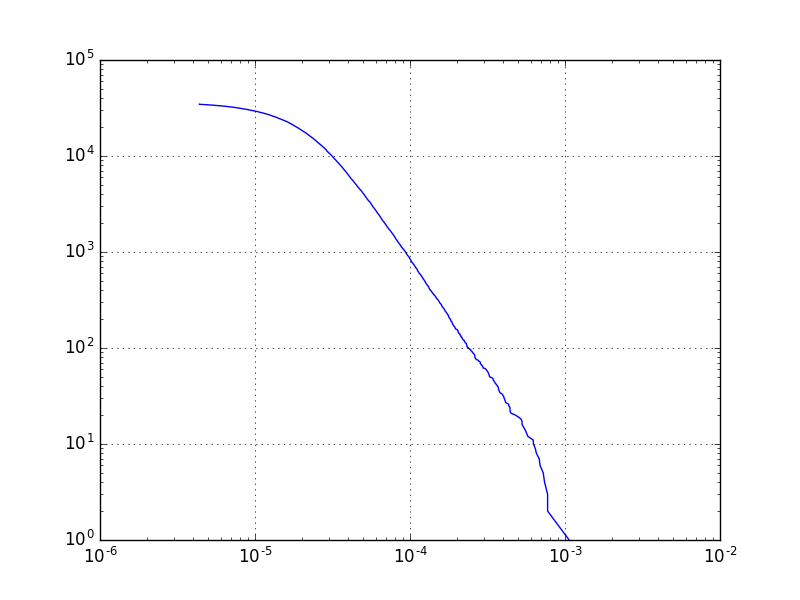
\includegraphics[width=\linewidth]{img/cit-HepPh/pagerank_ccdf.png}
  \caption*{cit-HepPh}
\endminipage\hfill
\minipage{0.33\textwidth}
  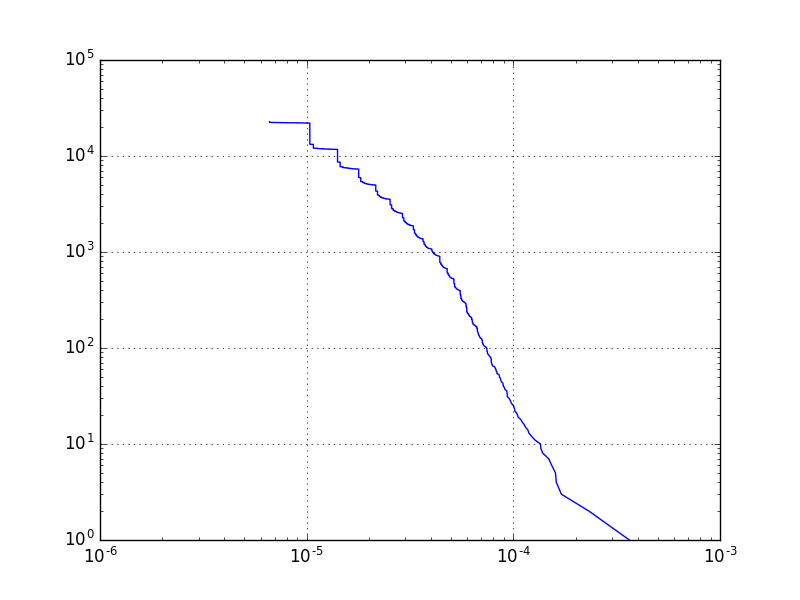
\includegraphics[width=\linewidth]{img/p2p-Gnutella25/pagerank_ccdf.png}
  \caption*{p2p-Gnutella25}
\endminipage\hfill
\minipage{0.33\textwidth}
  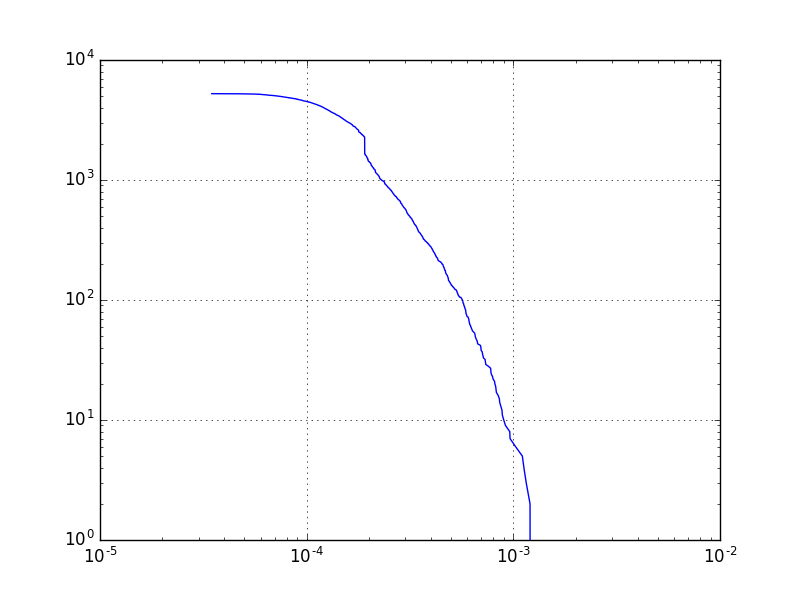
\includegraphics[width=\linewidth]{img/ca-GrQc/pagerank_ccdf.png}
  \caption*{ca-GrQc}
\endminipage
\end{figure}
\begin{figure}[H]
\minipage{0.33\textwidth}
  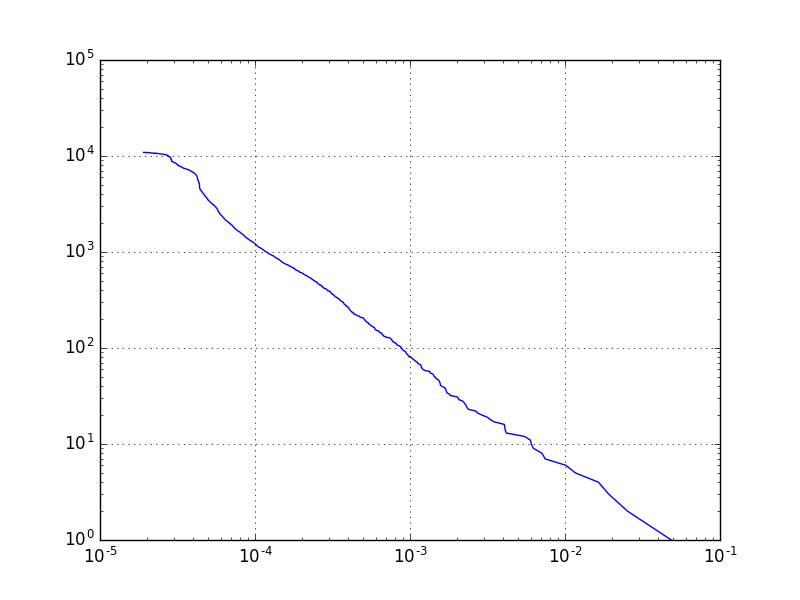
\includegraphics[width=\linewidth]{img/oregon-010331/pagerank_ccdf.png}
  \caption*{Oregon1-010331}
\endminipage\hfill
\minipage{0.33\textwidth}
  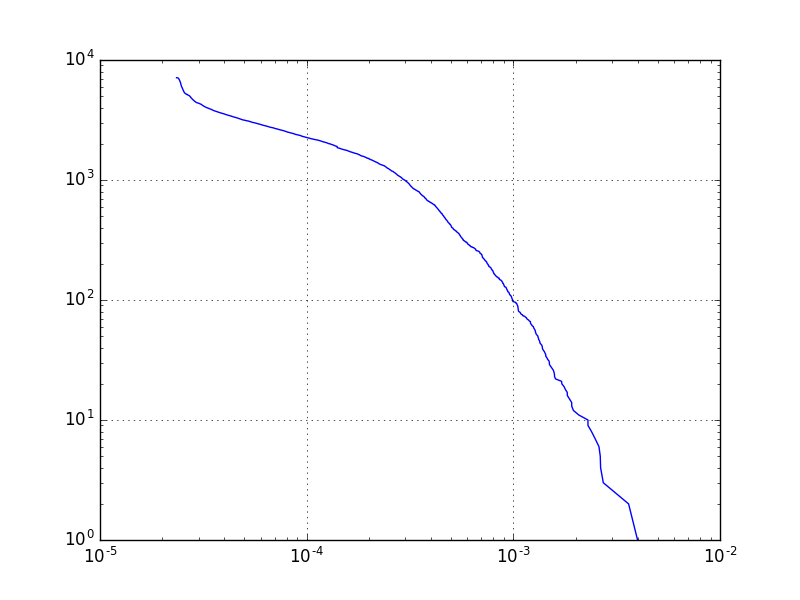
\includegraphics[width=\linewidth]{img/wiki-Vote/pagerank_ccdf.png}
  \caption*{wiki-Vote}
\endminipage\hfill
\minipage{0.33\textwidth}
  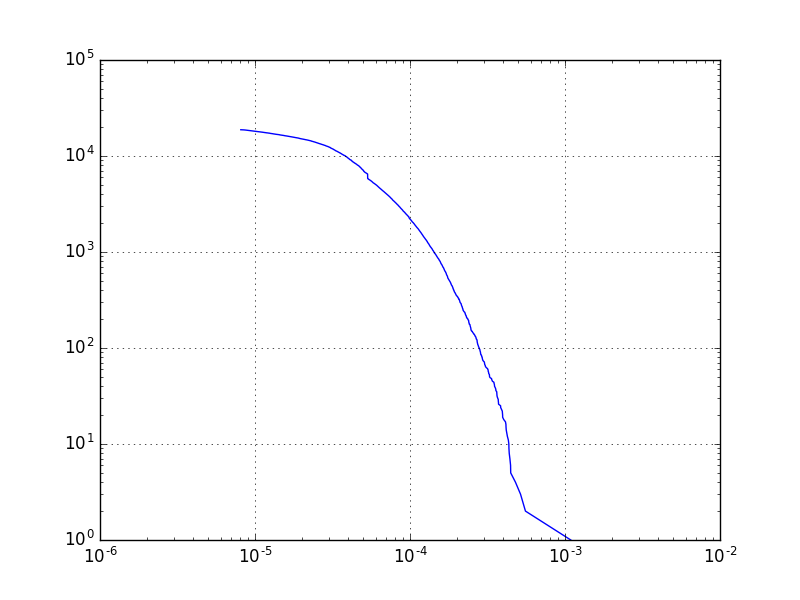
\includegraphics[width=\linewidth]{img/ca-Astro/pagerank_ccdf.png}
  \caption*{ca-Astro}
\endminipage
\end{figure}
\begin{figure}[H]
\minipage{0.33\textwidth}
  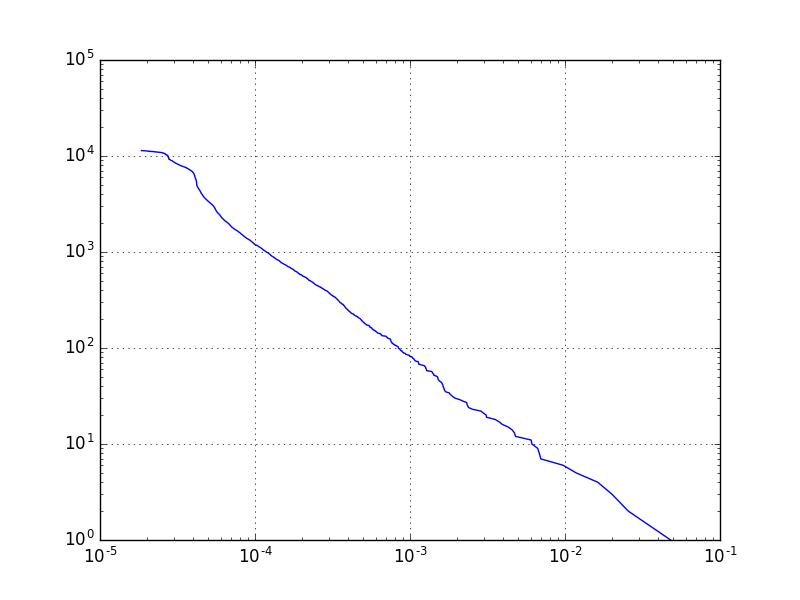
\includegraphics[width=\linewidth]{img/oregon-010519/pagerank_ccdf.png}
  \caption*{Oregon1-010519}
\endminipage\hfill
\minipage{0.33\textwidth}
  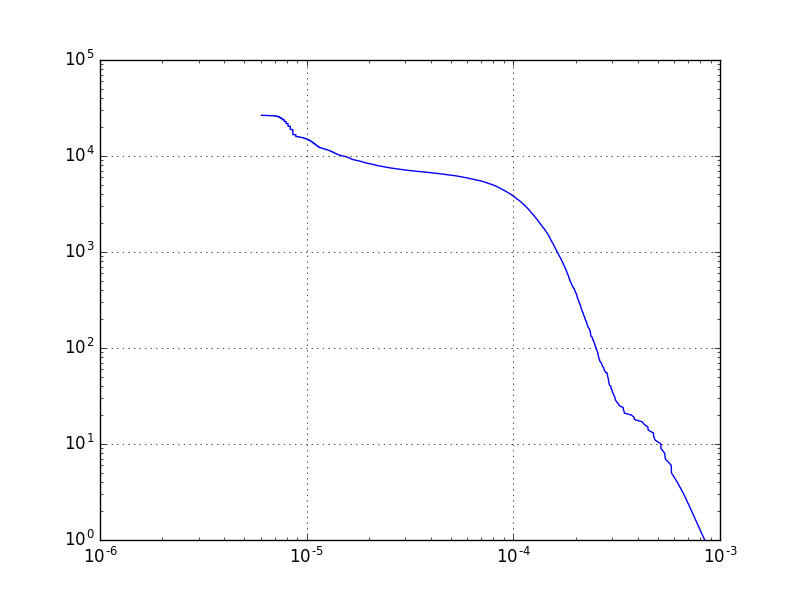
\includegraphics[width=\linewidth]{img/p2p-Gnutella24/pagerank_ccdf.png}
  \caption*{p2p-Gnutella24}
\endminipage\hfill
\minipage{0.33\textwidth}
  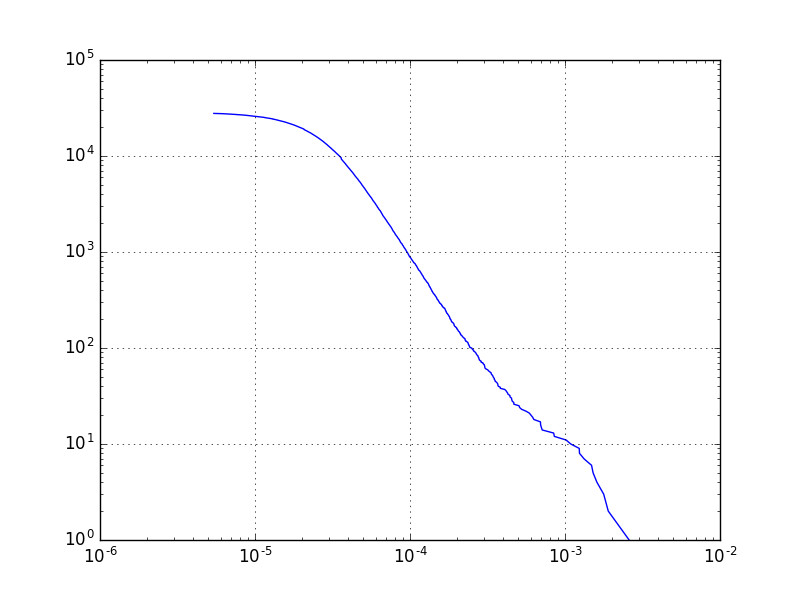
\includegraphics[width=\linewidth]{img/cit-HepTh/pagerank_ccdf.png}
  \caption*{cit-HepTh}
\endminipage
\end{figure}

Observations
\begin{itemize}
\item Via CCDF plots, we see many datasets follow power law between pagerank score and counts. This implies that only a few \texttt{'famous'} users own large impacts, while most \texttt{'ordinary'} users have small pagerank score $\sim [10^{-5}, 10^{-4}]$
\item However, for facebook dataset, the CCDF plot is not quite linear. This can be interpreted that a majority of Facebook users have low pagerank score and it is very hard to get pagerank score above a certain threshold.
\end{itemize}

\subsubsection{Eigen Value Distribution}

Scatter plot\quad x-axis: rank \quad y-axis: abs(eigen value)

\begin{figure}[H]
\minipage{0.33\textwidth}
  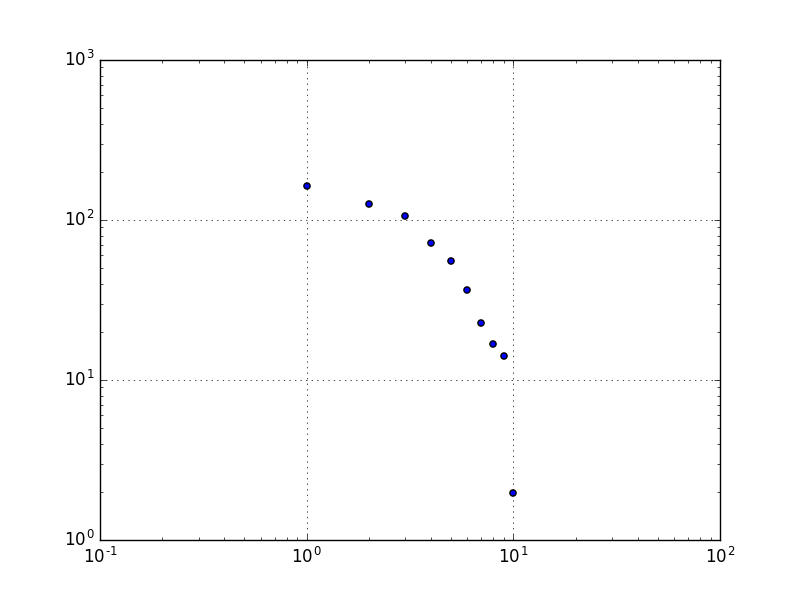
\includegraphics[width=\linewidth]{img/facebook/eig.png}
  \caption*{Facebook}
\endminipage\hfill
\minipage{0.33\textwidth}
  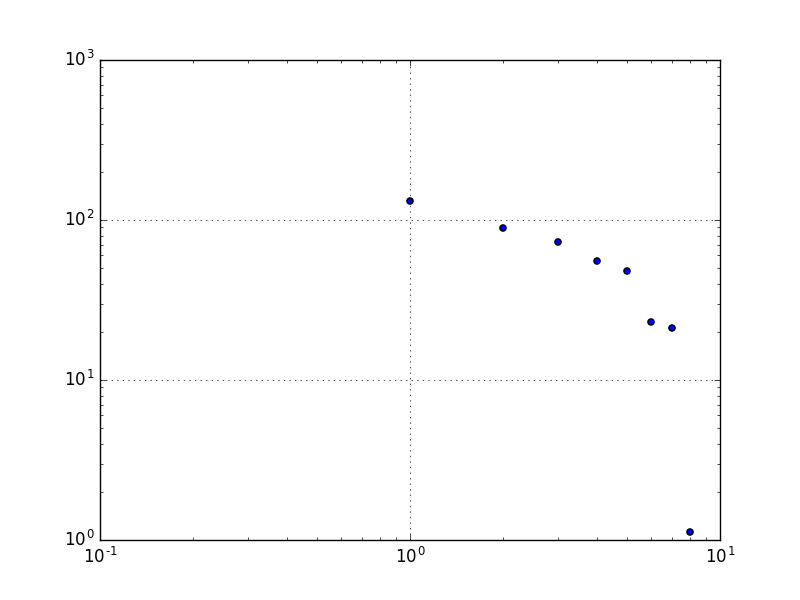
\includegraphics[width=\linewidth]{img/slashDot/eig.png}
  \caption*{soc-Slashdot0811}
\endminipage\hfill
\minipage{0.33\textwidth}
  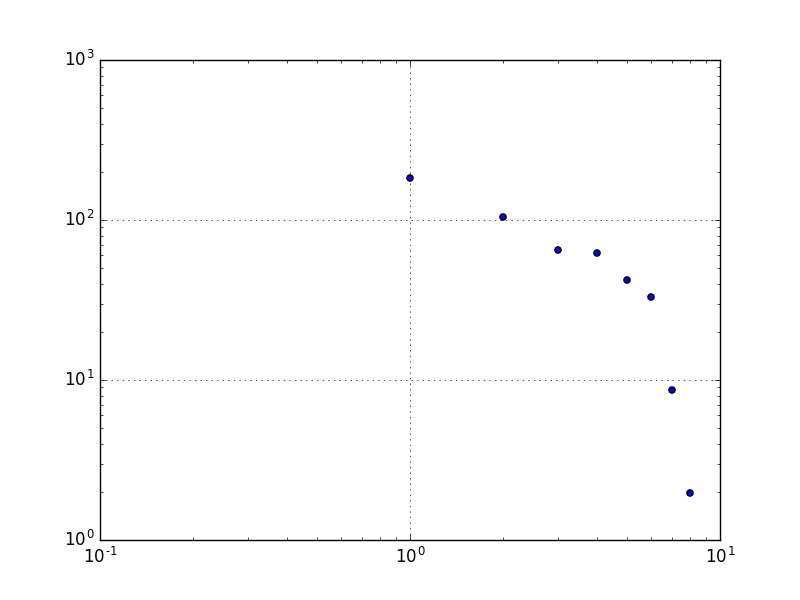
\includegraphics[width=\linewidth]{img/soc-E/eig.png}
  \caption*{soc-Epinions1}
\endminipage
\end{figure}
\begin{figure}[H]
\minipage{0.33\textwidth}
  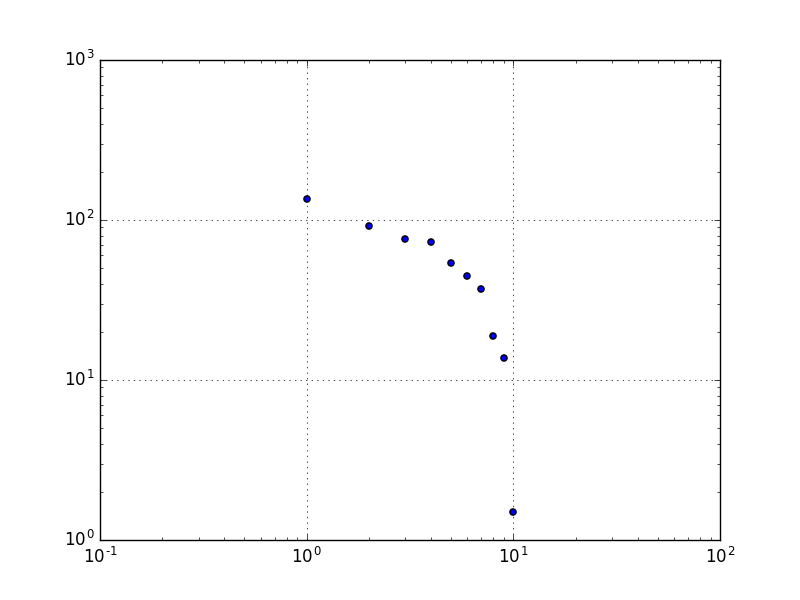
\includegraphics[width=\linewidth]{img/slashDot09/eig.png}
  \caption*{soc-Slashdot0922}
\endminipage\hfill
\minipage{0.33\textwidth}
  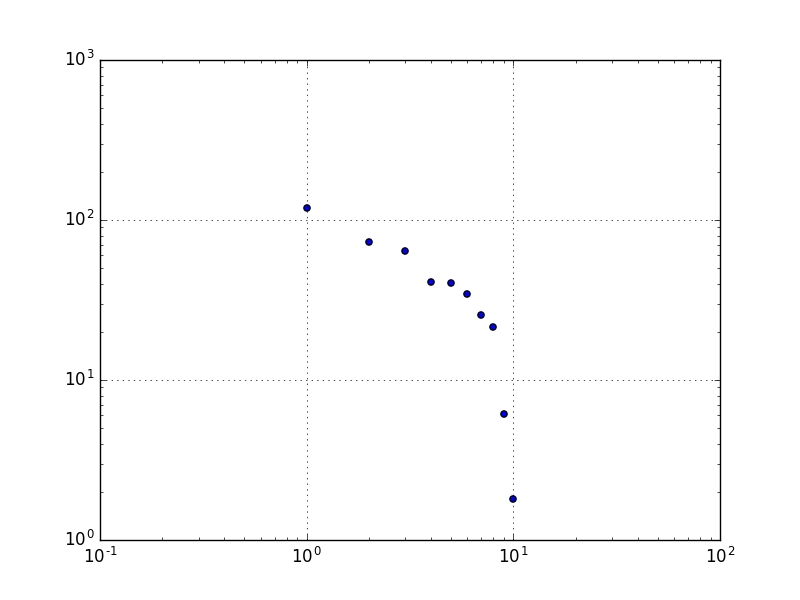
\includegraphics[width=\linewidth]{img/email/eig.png}
  \caption*{email-Enron}
\endminipage\hfill
\minipage{0.33\textwidth}
  \includegraphics[width=\linewidth]{img/ca-HepTh/eig.png}
  \caption*{ca-HepTh}
\endminipage
\end{figure}
\begin{figure}[H]
\minipage{0.33\textwidth}
  \includegraphics[width=\linewidth]{img/cit-HepPh/eig.png}
  \caption*{cit-HepPh}
\endminipage\hfill
\minipage{0.33\textwidth}
  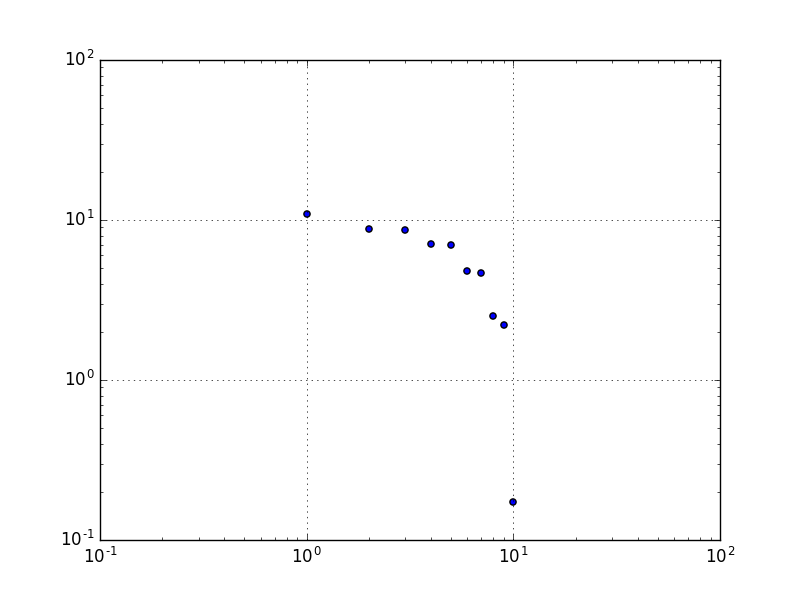
\includegraphics[width=\linewidth]{img/p2p-Gnutella25/eig.png}
  \caption*{p2p-Gnutella25}
\endminipage\hfill
\minipage{0.33\textwidth}
  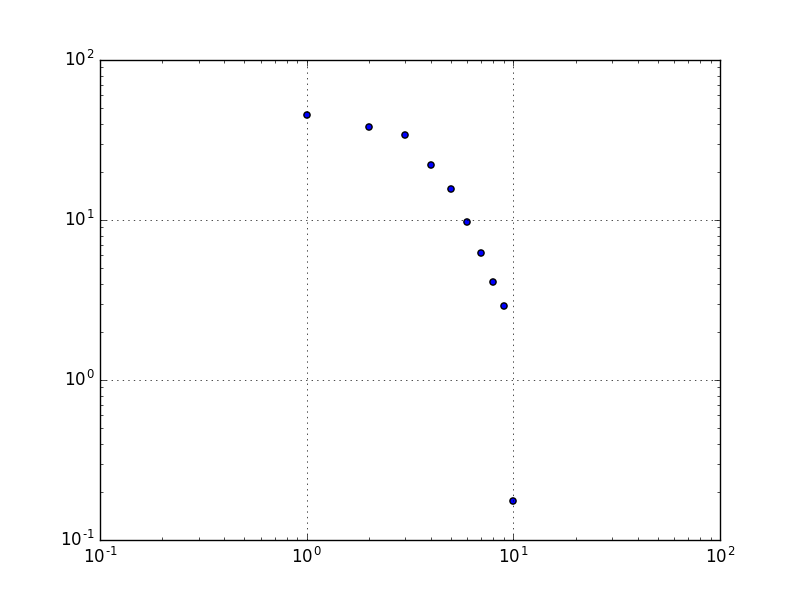
\includegraphics[width=\linewidth]{img/ca-GrQc/eig.png}
  \caption*{ca-GrQc}
\endminipage
\end{figure}
\begin{figure}[H]
\minipage{0.33\textwidth}
  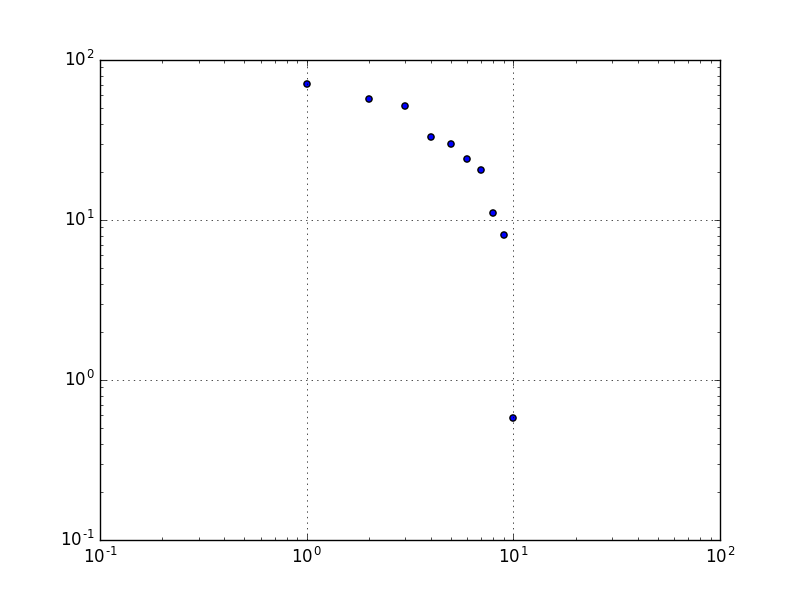
\includegraphics[width=\linewidth]{img/oregon-010331/eig.png}
  \caption*{Oregon1-010331}
\endminipage\hfill
\minipage{0.33\textwidth}
  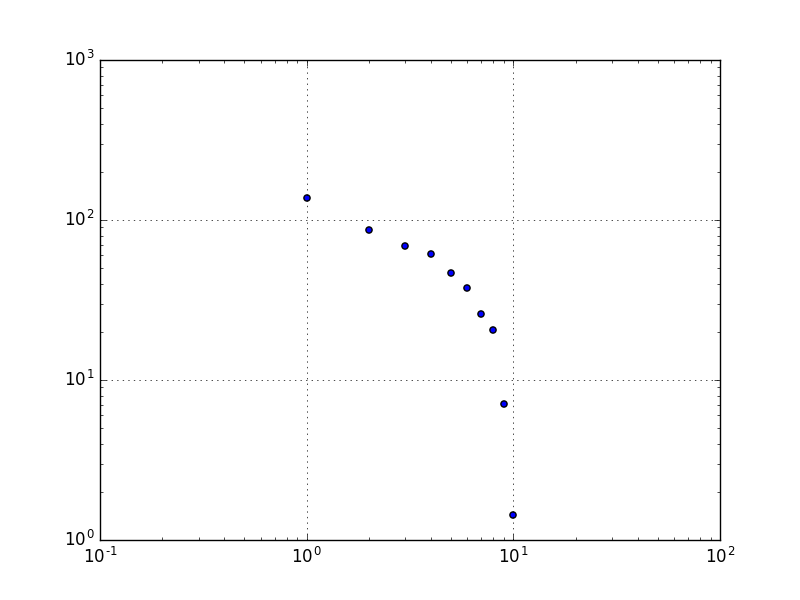
\includegraphics[width=\linewidth]{img/wiki-Vote/eig.png}
  \caption*{wiki-Vote}
\endminipage\hfill
\minipage{0.33\textwidth}
  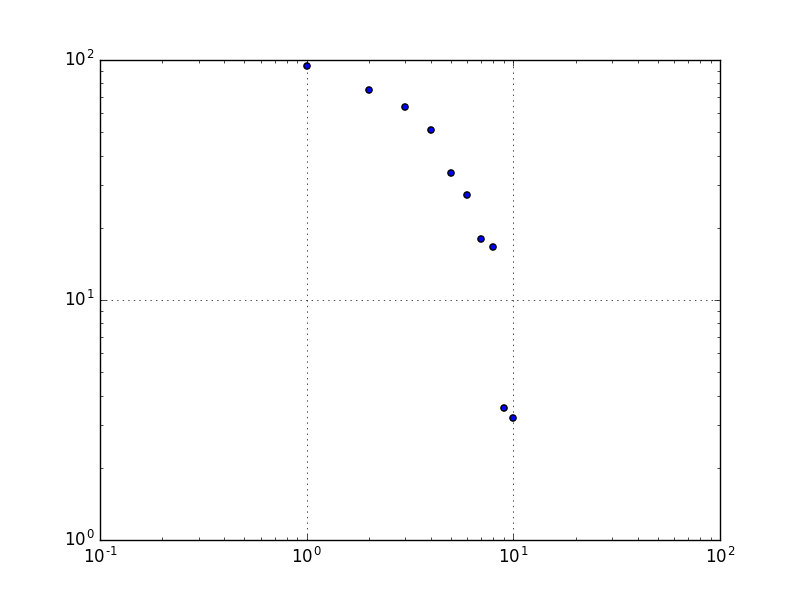
\includegraphics[width=\linewidth]{img/ca-Astro/eig.png}
  \caption*{ca-Astro}
\endminipage
\end{figure}
\begin{figure}[H]
\minipage{0.33\textwidth}
  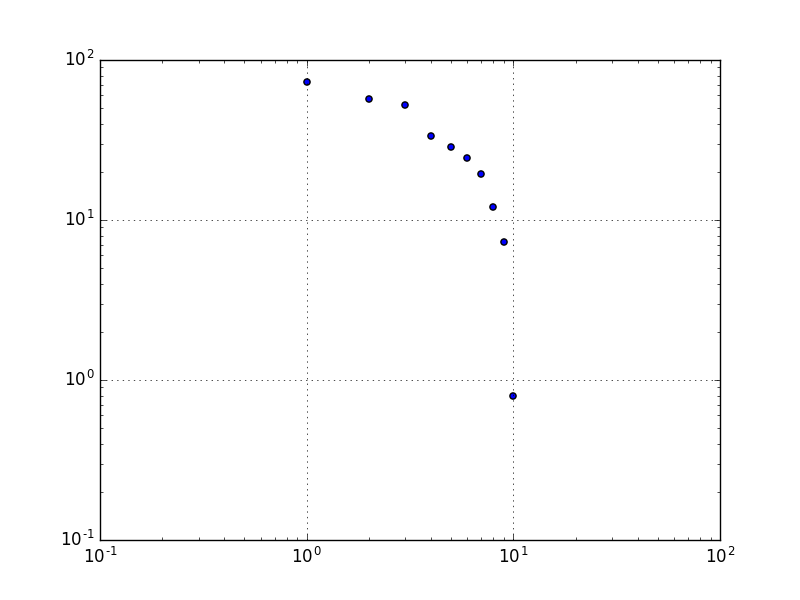
\includegraphics[width=\linewidth]{img/oregon-010519/eig.png}
  \caption*{Oregon1-010519}
\endminipage\hfill
\minipage{0.33\textwidth}
  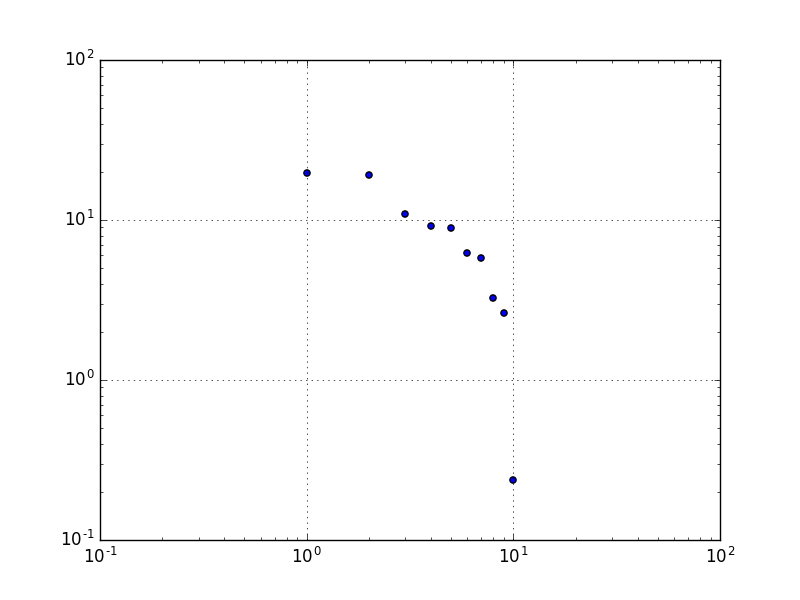
\includegraphics[width=\linewidth]{img/p2p-Gnutella24/eig.png}
  \caption*{p2p-Gnutella24}
\endminipage\hfill
\minipage{0.33\textwidth}
  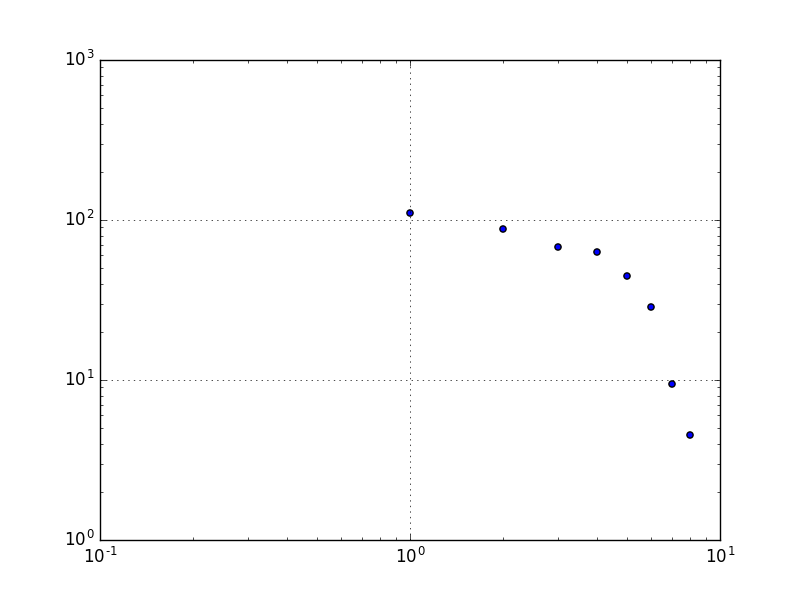
\includegraphics[width=\linewidth]{img/cit-HepTh/eig.png}
  \caption*{cit-HepTh}
\endminipage
\end{figure}

Observations
\begin{itemize}
\item We draw the top 10 eigen values of each dataset. It can be seen that \texttt{\{eigen value $\lambda_i$ - rank $i$\}} follows power law for most datasets.
\item Eigen value drops dramatically at rank 8, rank 9 and rank 10. It takes much longer time to converge for the calculation of these eigen values and their values are $\sim [0.1, 1]$. This implies that we can actually compress many realworld datasets with top 8 eigen values and eigen vectors without losing much information.
\end{itemize}

\subsubsection{Connected-component-size distribution}

Scatter plot\quad x-axis: component size \quad y-axis: count

\begin{figure}[H]
\minipage{0.33\textwidth}
  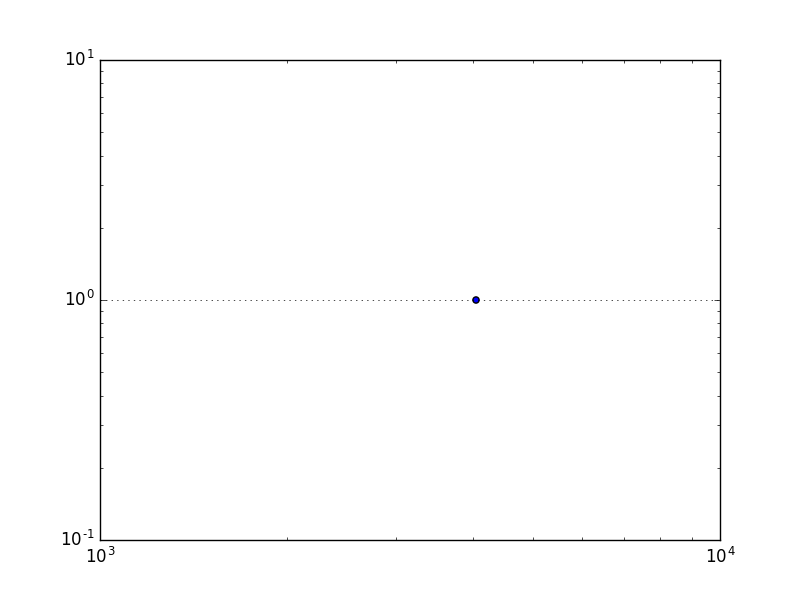
\includegraphics[width=\linewidth]{img/facebook/comp_dist.png}
  \caption*{Facebook}
\endminipage\hfill
\minipage{0.33\textwidth}
  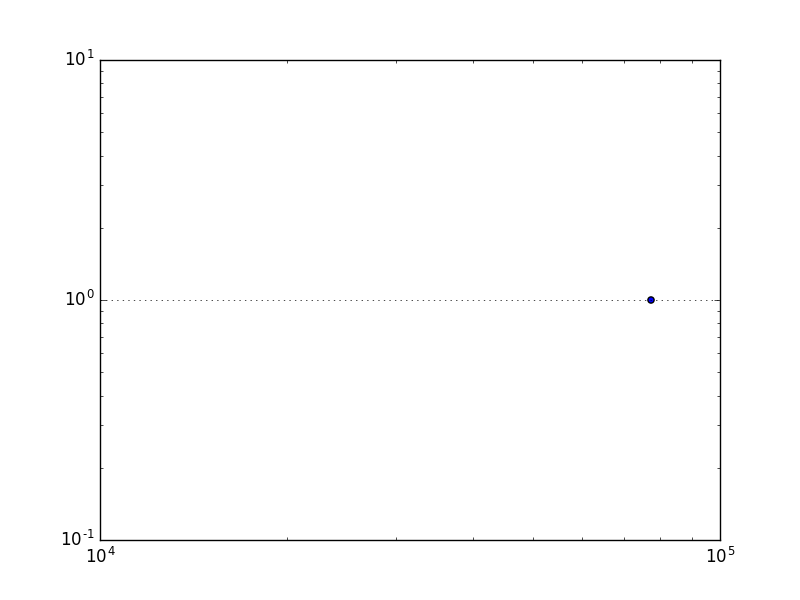
\includegraphics[width=\linewidth]{img/slashDot/comp_dist.png}
  \caption*{soc-Slashdot0811}
\endminipage\hfill
\minipage{0.33\textwidth}
  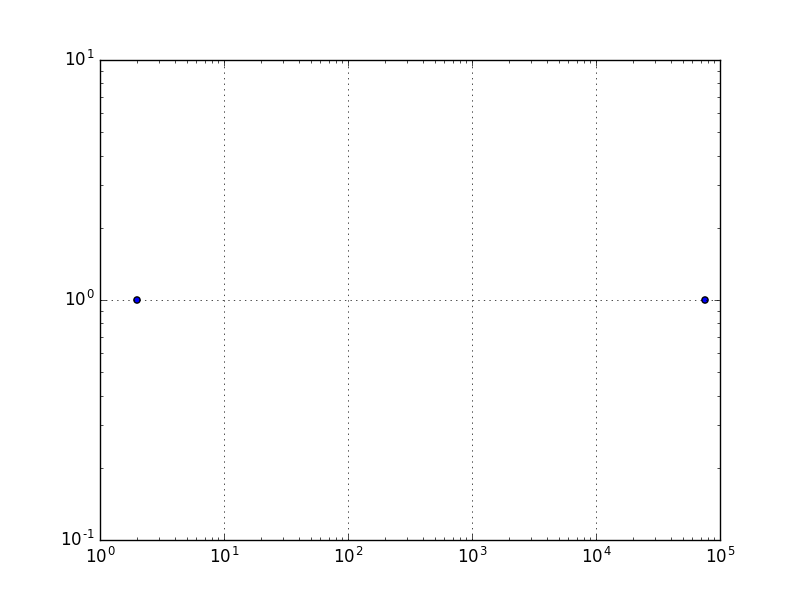
\includegraphics[width=\linewidth]{img/soc-E/comp_dist.png}
  \caption*{soc-Epinions1}
\endminipage
\end{figure}
\begin{figure}[H]
\minipage{0.33\textwidth}
  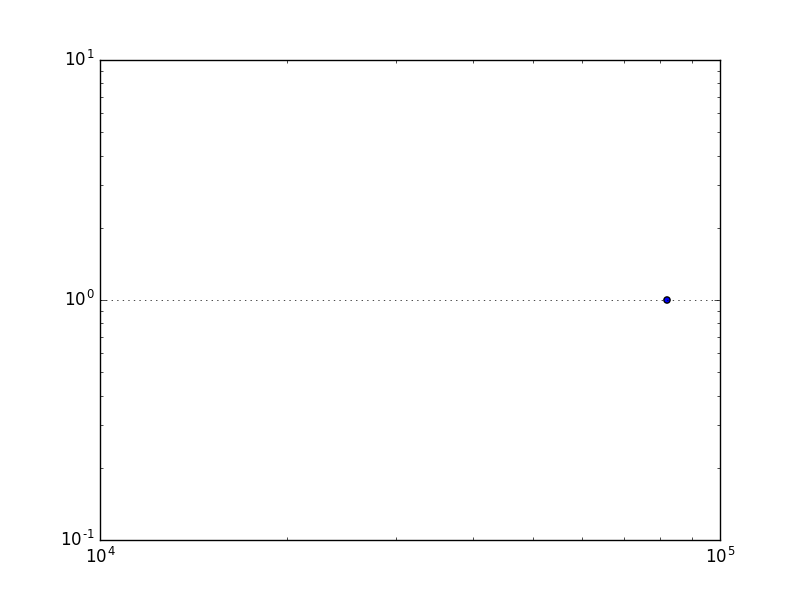
\includegraphics[width=\linewidth]{img/slashDot09/comp_dist.png}
  \caption*{soc-Slashdot0922}
\endminipage\hfill
\minipage{0.33\textwidth}
  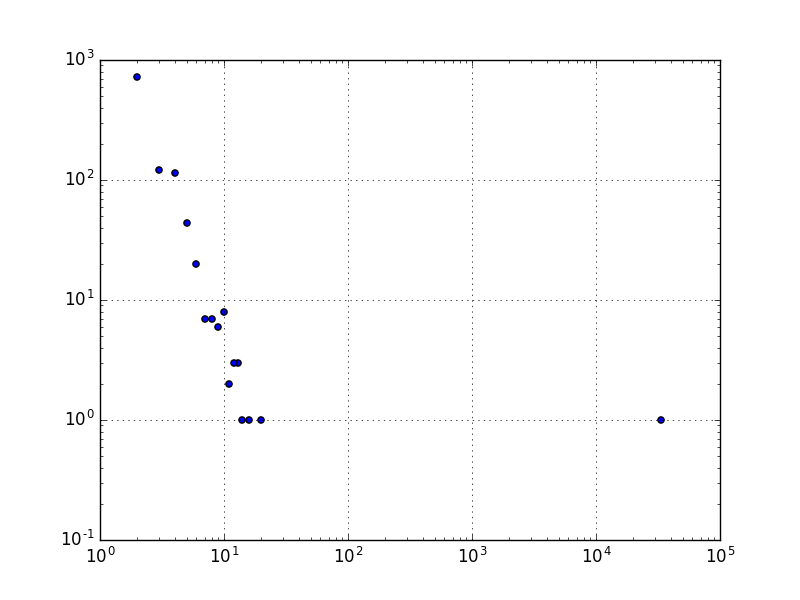
\includegraphics[width=\linewidth]{img/email/comp_dist.png}
  \caption*{email-Enron}
\endminipage\hfill
\minipage{0.33\textwidth}
  \includegraphics[width=\linewidth]{img/ca-HepTh/comp_dist.png}
  \caption*{ca-HepTh}
\endminipage
\end{figure}
\begin{figure}[H]
\minipage{0.33\textwidth}
  \includegraphics[width=\linewidth]{img/cit-HepPh/comp_dist.png}
  \caption*{cit-HepPh}
\endminipage\hfill
\minipage{0.33\textwidth}
  \includegraphics[width=\linewidth]{img/p2p-Gnutella25/comp_dist.png}
  \caption*{p2p-Gnutella25}
\endminipage\hfill
\minipage{0.33\textwidth}
  \includegraphics[width=\linewidth]{img/ca-GrQc/comp_dist.png}
  \caption*{ca-GrQc}
\endminipage
\end{figure}
\begin{figure}[H]
\minipage{0.33\textwidth}
  \includegraphics[width=\linewidth]{img/oregon-010331/comp_dist.png}
  \caption*{Oregon1-010331}
\endminipage\hfill
\minipage{0.33\textwidth}
  \includegraphics[width=\linewidth]{img/wiki-Vote/comp_dist.png}
  \caption*{wiki-Vote}
\endminipage\hfill
\minipage{0.33\textwidth}
  \includegraphics[width=\linewidth]{img/ca-Astro/comp_dist.png}
  \caption*{ca-Astro}
\endminipage
\end{figure}
\begin{figure}[H]
\minipage{0.33\textwidth}
  \includegraphics[width=\linewidth]{img/oregon-010519/comp_dist.png}
  \caption*{Oregon1-010519}
\endminipage\hfill
\minipage{0.33\textwidth}
  \includegraphics[width=\linewidth]{img/p2p-Gnutella24/comp_dist.png}
  \caption*{p2p-Gnutella24}
\endminipage\hfill
\minipage{0.33\textwidth}
  \includegraphics[width=\linewidth]{img/cit-HepTh/comp_dist.png}
  \caption*{cit-HepTh}
\endminipage
\end{figure}

Observations
\begin{itemize}
\item \textbf{Social networks} (Facebook, soc-Slashdot, soc-Epinions), \textbf{P2P networks} (p2p-Gnutella) and \textbf{Autonomous networks} (Oregon1) are very well and fully connected, resulting in only one or two connected components.
\item Other networks such as \textbf{Collaboration networks} and \textbf{Citation networks} exhibits a power law relation for components of small \& medium sizes. For these networks, there exists one large component whose size is greater than sum of the rest. 
\end{itemize}


\subsubsection{Coreness Value Distribution}

Scatter plot\quad x-axis: k-core value \quad y-axis: count

\begin{figure}[H]
\minipage{0.33\textwidth}
  \includegraphics[width=\linewidth]{img/facebook/kcore_dist.png}
  \caption*{Facebook}
\endminipage\hfill
\minipage{0.33\textwidth}
  \includegraphics[width=\linewidth]{img/slashDot/kcore_dist.png}
  \caption*{soc-Slashdot0811}
\endminipage\hfill
\minipage{0.33\textwidth}
  \includegraphics[width=\linewidth]{img/soc-E/kcore_dist.png}
  \caption*{soc-Epinions1}
\endminipage
\end{figure}
\begin{figure}[H]
\minipage{0.33\textwidth}
  \includegraphics[width=\linewidth]{img/slashDot09/kcore_dist.png}
  \caption*{soc-Slashdot0922}
\endminipage\hfill
\minipage{0.33\textwidth}
  \includegraphics[width=\linewidth]{img/email/kcore_dist.png}
  \caption*{email-Enron}
\endminipage\hfill
\minipage{0.33\textwidth}
  \includegraphics[width=\linewidth]{img/ca-HepTh/kcore_dist.png}
  \caption*{ca-HepTh}
\endminipage
\end{figure}
\begin{figure}[H]
\minipage{0.33\textwidth}
  \includegraphics[width=\linewidth]{img/cit-HepPh/kcore_dist.png}
  \caption*{cit-HepPh}
\endminipage\hfill
\minipage{0.33\textwidth}
  \includegraphics[width=\linewidth]{img/p2p-Gnutella25/kcore_dist.png}
  \caption*{p2p-Gnutella25}
\endminipage\hfill
\minipage{0.33\textwidth}
  \includegraphics[width=\linewidth]{img/ca-GrQc/kcore_dist.png}
  \caption*{ca-GrQc}
\endminipage
\end{figure}
\begin{figure}[H]
\minipage{0.33\textwidth}
  \includegraphics[width=\linewidth]{img/oregon-010331/kcore_dist.png}
  \caption*{Oregon1-010331}
\endminipage\hfill
\minipage{0.33\textwidth}
  \includegraphics[width=\linewidth]{img/wiki-Vote/kcore_dist.png}
  \caption*{wiki-Vote}
\endminipage\hfill
\minipage{0.33\textwidth}
  \includegraphics[width=\linewidth]{img/ca-Astro/kcore_dist.png}
  \caption*{ca-Astro}
\endminipage
\end{figure}
\begin{figure}[H]
\minipage{0.33\textwidth}
  \includegraphics[width=\linewidth]{img/oregon-010519/kcore_dist.png}
  \caption*{Oregon1-010519}
\endminipage\hfill
\minipage{0.33\textwidth}
  \includegraphics[width=\linewidth]{img/p2p-Gnutella24/kcore_dist.png}
  \caption*{p2p-Gnutella24}
\endminipage\hfill
\minipage{0.33\textwidth}
  \includegraphics[width=\linewidth]{img/cit-HepTh/kcore_dist.png}
  \caption*{cit-HepTh}
\endminipage
\end{figure}

Observations
\begin{itemize}
\item Most datasets follow power law between \texttt{kcore value - count}.
\item It is easy to spot some outliers in dataset soc-Slashdot. soc-Slashdot graph has several dozen nodes whose k-core value are 1, loosely connected with other nodes.
\end{itemize}

\subsubsection{Radius Distribution}

PDF\quad x-axis: raidus \quad y-axis: count

\begin{figure}[H]
\minipage{0.33\textwidth}
  \includegraphics[width=\linewidth]{img/facebook/radius_dist.png}
  \caption*{Facebook}
\endminipage\hfill
\minipage{0.33\textwidth}
  \includegraphics[width=\linewidth]{img/slashDot/radius_dist.png}
  \caption*{soc-Slashdot0811}
\endminipage\hfill
\minipage{0.33\textwidth}
  \includegraphics[width=\linewidth]{img/soc-E/radius_dist.png}
  \caption*{soc-Epinions1}
\endminipage
\end{figure}
\begin{figure}[H]
\minipage{0.33\textwidth}
  \includegraphics[width=\linewidth]{img/slashDot09/radius_dist.png}
  \caption*{soc-Slashdot0922}
\endminipage\hfill
\minipage{0.33\textwidth}
  \includegraphics[width=\linewidth]{img/email/radius_dist.png}
  \caption*{email-Enron}
\endminipage\hfill
\minipage{0.33\textwidth}
  \includegraphics[width=\linewidth]{img/ca-HepTh/radius_dist.png}
  \caption*{ca-HepTh}
\endminipage
\end{figure}
\begin{figure}[H]
\minipage{0.33\textwidth}
  \includegraphics[width=\linewidth]{img/cit-HepPh/radius_dist.png}
  \caption*{cit-HepPh}
\endminipage\hfill
\minipage{0.33\textwidth}
  \includegraphics[width=\linewidth]{img/p2p-Gnutella25/radius_dist.png}
  \caption*{p2p-Gnutella25}
\endminipage\hfill
\minipage{0.33\textwidth}
  \includegraphics[width=\linewidth]{img/ca-GrQc/radius_dist.png}
  \caption*{ca-GrQc}
\endminipage
\end{figure}
\begin{figure}[H]
\minipage{0.33\textwidth}
  \includegraphics[width=\linewidth]{img/oregon-010331/radius_dist.png}
  \caption*{Oregon1-010331}
\endminipage\hfill
\minipage{0.33\textwidth}
  \includegraphics[width=\linewidth]{img/wiki-Vote/radius_dist.png}
  \caption*{wiki-Vote}
\endminipage\hfill
\minipage{0.33\textwidth}
  \includegraphics[width=\linewidth]{img/ca-Astro/radius_dist.png}
  \caption*{ca-Astro}
\endminipage
\end{figure}
\begin{figure}[H]
\minipage{0.33\textwidth}
  \includegraphics[width=\linewidth]{img/oregon-010519/radius_dist.png}
  \caption*{Oregon1-010519}
\endminipage\hfill
\minipage{0.33\textwidth}
  \includegraphics[width=\linewidth]{img/p2p-Gnutella24/radius_dist.png}
  \caption*{p2p-Gnutella24}
\endminipage\hfill
\minipage{0.33\textwidth}
  \includegraphics[width=\linewidth]{img/cit-HepTh/radius_dist.png}
  \caption*{cit-HepTh}
\endminipage
\end{figure}

Observations
\begin{itemize}
\item Realworld graphs have small diameters. Most nodes follow \textbf{six degree principle} (their effective radius are 5-7). 
\item We see that radius distribution (in PDF graph) is multimodal.
\end{itemize}

\subsubsection{Degree VS PageRank Distribution}

Scatter plot\quad a-axis: degree \quad y-axis: pagerank score

\begin{figure}[H]
\minipage{0.33\textwidth}
  \includegraphics[width=\linewidth]{img/facebook/degreeVSpagerank.png}
  \caption*{Facebook}
\endminipage\hfill
\minipage{0.33\textwidth}
  \includegraphics[width=\linewidth]{img/slashDot/degreeVSpagerank.png}
  \caption*{soc-Slashdot0811}
\endminipage\hfill
\minipage{0.33\textwidth}
  \includegraphics[width=\linewidth]{img/soc-E/degreeVSpagerank.png}
  \caption*{soc-Epinions1}
\endminipage
\end{figure}
\begin{figure}[H]
\minipage{0.33\textwidth}
  \includegraphics[width=\linewidth]{img/slashDot09/degreeVSpagerank.png}
  \caption*{soc-Slashdot0922}
\endminipage\hfill
\minipage{0.33\textwidth}
  \includegraphics[width=\linewidth]{img/email/degreeVSpagerank.png}
  \caption*{email-Enron}
\endminipage\hfill
\minipage{0.33\textwidth}
  \includegraphics[width=\linewidth]{img/ca-HepTh/degreeVSpagerank.png}
  \caption*{ca-HepTh}
\endminipage
\end{figure}
\begin{figure}[H]
\minipage{0.33\textwidth}
  \includegraphics[width=\linewidth]{img/cit-HepPh/degreeVSpagerank.png}
  \caption*{cit-HepPh}
\endminipage\hfill
\minipage{0.33\textwidth}
  \includegraphics[width=\linewidth]{img/p2p-Gnutella25/degreeVSpagerank.png}
  \caption*{p2p-Gnutella25}
\endminipage\hfill
\minipage{0.33\textwidth}
  \includegraphics[width=\linewidth]{img/ca-GrQc/degreeVSpagerank.png}
  \caption*{ca-GrQc}
\endminipage
\end{figure}
\begin{figure}[H]
\minipage{0.33\textwidth}
  \includegraphics[width=\linewidth]{img/oregon-010331/degreeVSpagerank.png}
  \caption*{Oregon1-010331}
\endminipage\hfill
\minipage{0.33\textwidth}
  \includegraphics[width=\linewidth]{img/wiki-Vote/degreeVSpagerank.png}
  \caption*{wiki-Vote}
\endminipage\hfill
\minipage{0.33\textwidth}
  \includegraphics[width=\linewidth]{img/ca-Astro/degreeVSpagerank.png}
  \caption*{ca-Astro}
\endminipage
\end{figure}
\begin{figure}[H]
\minipage{0.33\textwidth}
  \includegraphics[width=\linewidth]{img/oregon-010519/degreeVSpagerank.png}
  \caption*{Oregon1-010519}
\endminipage\hfill
\minipage{0.33\textwidth}
  \includegraphics[width=\linewidth]{img/p2p-Gnutella24/degreeVSpagerank.png}
  \caption*{p2p-Gnutella24}
\endminipage\hfill
\minipage{0.33\textwidth}
  \includegraphics[width=\linewidth]{img/cit-HepTh/degreeVSpagerank.png}
  \caption*{cit-HepTh}
\endminipage
\end{figure}

Observations
\begin{itemize}
\item In log-log scale, degree and pagerank score are positively correlated and approximately growing linearly.
\item \textbf{P2P networks} and \textbf{collaboration networks} are much more sparse and scattered compared to others. 
\item Some datasets e.g.\texttt{cit-HepPh}, we can observe that pagerank score grows super-linearly with degree. This means that growing connections can bring in even bigger impacts.
\end{itemize}

\subsubsection{Degree VS Coreness Distribution}

Scatter plot\quad x-axis: degree \quad y-axis: k-core value

\begin{figure}[H]
\minipage{0.33\textwidth}
  \includegraphics[width=\linewidth]{img/facebook/degreeVSkcore.png}
  \caption*{Facebook}
\endminipage\hfill
\minipage{0.33\textwidth}
  \includegraphics[width=\linewidth]{img/slashDot/degreeVSkcore.png}
  \caption*{soc-Slashdot0811}
\endminipage\hfill
\minipage{0.33\textwidth}
  \includegraphics[width=\linewidth]{img/soc-E/degreeVSkcore.png}
  \caption*{soc-Epinions1}
\endminipage
\end{figure}
\begin{figure}[H]
\minipage{0.33\textwidth}
  \includegraphics[width=\linewidth]{img/slashDot09/degreeVSkcore.png}
  \caption*{soc-Slashdot0922}
\endminipage\hfill
\minipage{0.33\textwidth}
  \includegraphics[width=\linewidth]{img/email/degreeVSkcore.png}
  \caption*{email-Enron}
\endminipage\hfill
\minipage{0.33\textwidth}
  \includegraphics[width=\linewidth]{img/ca-HepTh/degreeVSkcore.png}
  \caption*{ca-HepTh}
\endminipage
\end{figure}
\begin{figure}[H]
\minipage{0.33\textwidth}
  \includegraphics[width=\linewidth]{img/cit-HepPh/degreeVSkcore.png}
  \caption*{cit-HepPh}
\endminipage\hfill
\minipage{0.33\textwidth}
  \includegraphics[width=\linewidth]{img/p2p-Gnutella25/degreeVSkcore.png}
  \caption*{p2p-Gnutella25}
\endminipage\hfill
\minipage{0.33\textwidth}
  \includegraphics[width=\linewidth]{img/ca-GrQc/degreeVSkcore.png}
  \caption*{ca-GrQc}
\endminipage
\end{figure}
\begin{figure}[H]
\minipage{0.33\textwidth}
  \includegraphics[width=\linewidth]{img/oregon-010331/degreeVSkcore.png}
  \caption*{Oregon1-010331}
\endminipage\hfill
\minipage{0.33\textwidth}
  \includegraphics[width=\linewidth]{img/wiki-Vote/degreeVSkcore.png}
  \caption*{wiki-Vote}
\endminipage\hfill
\minipage{0.33\textwidth}
  \includegraphics[width=\linewidth]{img/ca-Astro/degreeVSkcore.png}
  \caption*{ca-Astro}
\endminipage
\end{figure}
\begin{figure}[H]
\minipage{0.33\textwidth}
  \includegraphics[width=\linewidth]{img/oregon-010519/degreeVSkcore.png}
  \caption*{Oregon1-010519}
\endminipage\hfill
\minipage{0.33\textwidth}
  \includegraphics[width=\linewidth]{img/p2p-Gnutella24/degreeVSkcore.png}
  \caption*{p2p-Gnutella24}
\endminipage\hfill
\minipage{0.33\textwidth}
  \includegraphics[width=\linewidth]{img/cit-HepTh/degreeVSkcore.png}
  \caption*{cit-HepTh}
\endminipage
\end{figure}

Observations
\begin{itemize}
\item Like previous sections, degree VS coreness follows the same trend. Node's degree and kcore value are positively correlated and growing linearly. 
\item \textbf{P2P networks} and \textbf{collaboration networks} are not as dense as others. For such networks, kcore values and degree values are much more limited in a small range.
\end{itemize}

\subsection{Conclusions}

We have provided over 15 observations in the above sections. In general, we see find most graphs follow the power law either in scatter / PDF / CCDF form, i.e. a majority of nodes have low degrees / pagerank scores / k-core values. We also spotted some anomolies from plots. 

\section{Labor Division}

\begin{itemize}
\item Yuwei Zhang: Degree distribution, Eigen Value distribution, Radius Distribution, Degree VS PageRank Distribution
\item Silun Wang: Pagerank Distribution, Connected-component-size Distribution, Coreness Value Distribution, Degree VS Coreness Distribution
\end{itemize}

\section{Acknowledgement}

We would like to thank Nijith Jacob and Sharif Doghmi for their previous work on Graph Miner toolset. We also acknowledge SNAP for the dataset.
